\documentclass[10pt]{beamer}

\usepackage{style-custom}


\title{Superfluid properties of exciton polariton condensates in planar microcavities}
\subtitle{Colloquio IV anno}
\author[Carmelo Mordini]{Carmelo Mordini\\ \vspace{.7cm}
{\footnotesize Supervisors\\ \vspace{-.1cm}I. Carusotto ~ R. Fazio}}

\institute[SNS]
{
  Scuola Normale Superiore\\
  %University of Somewhere
  }
\date{Maggio 2014}


% % Delete this, if you do not want the table of contents to pop up at
% % the beginning of each subsection:
% \AtBeginSubsection[]
% {
%   \begin{frame}<beamer>{Riassunto}
%     \tableofcontents[currentsection,currentsubsection]
%   \end{frame}
% }

% Let's get started


\begin{document}

\begin{frame}
  \titlepage
\end{frame}

\begin{frame}{Outline}
  \tableofcontents[pausesections]
  % You might wish to add the option [pausesections]
\end{frame}

% Section and subsections will appear in the presentation overview
% and table of contents.
\section{Cavità di semiconduttori}

\subsection{Dinamica dei polaritoni}
% %  \begin{frame}{Cavità 2D}{fuffa}
%  \transwipe[direction=270]
%  \small
% % \begin{minipage}{\textwidth}
%   \begin{columns}
%
%   \begin{column}{.6\textwidth}
%     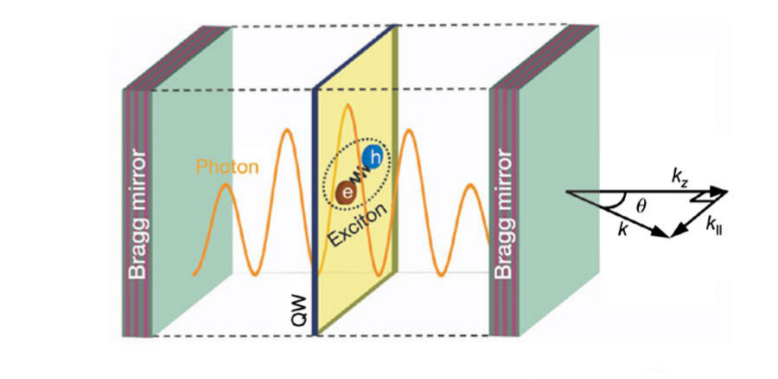
\includegraphics[width=\columnwidth]{pics/QW_color.png}
%   \end{column}
% %   \begin{column}{.4\textwidth}
%     Le cavità bidimensionali di semiconduttore si rivelano uno strumento potente per studiare la fisica dei fluidi quantistici.
%     \end{column}
%   \end{columns}
%   \end{minipage}
%
%   Il confinamento spaziale e l'interazione con il mezzo fanno acquistare alla luce una dinamica analoga a quella di un fluido di particelle.
%
%   \begin{minipage}{\textwidth}
%   \begin{columns}
%
%   \begin{column}{.3\textwidth}
%     \begin{itemize}
%      \item Interazioni luce-materia
%      \item Effetti macroscopici
%      \item Esperimenti
%     \end{itemize}
% %   \end{column}
% \hfill
%   \begin{column}{.5\textwidth}
%   \begin{figure}
%     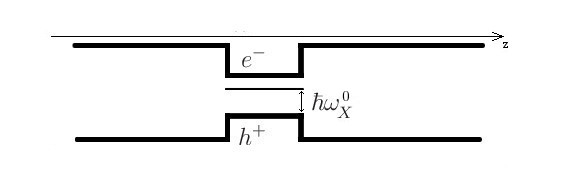
\includegraphics[width=\columnwidth]{pics/QW.jpg}
%   \end{figure}
%     \end{column}
%   \end{columns}
%   \end{minipage}
%
%
%  \end{frame}


\begin{frame}{Cavità 2D}

  \begin{figure}
     \fbox{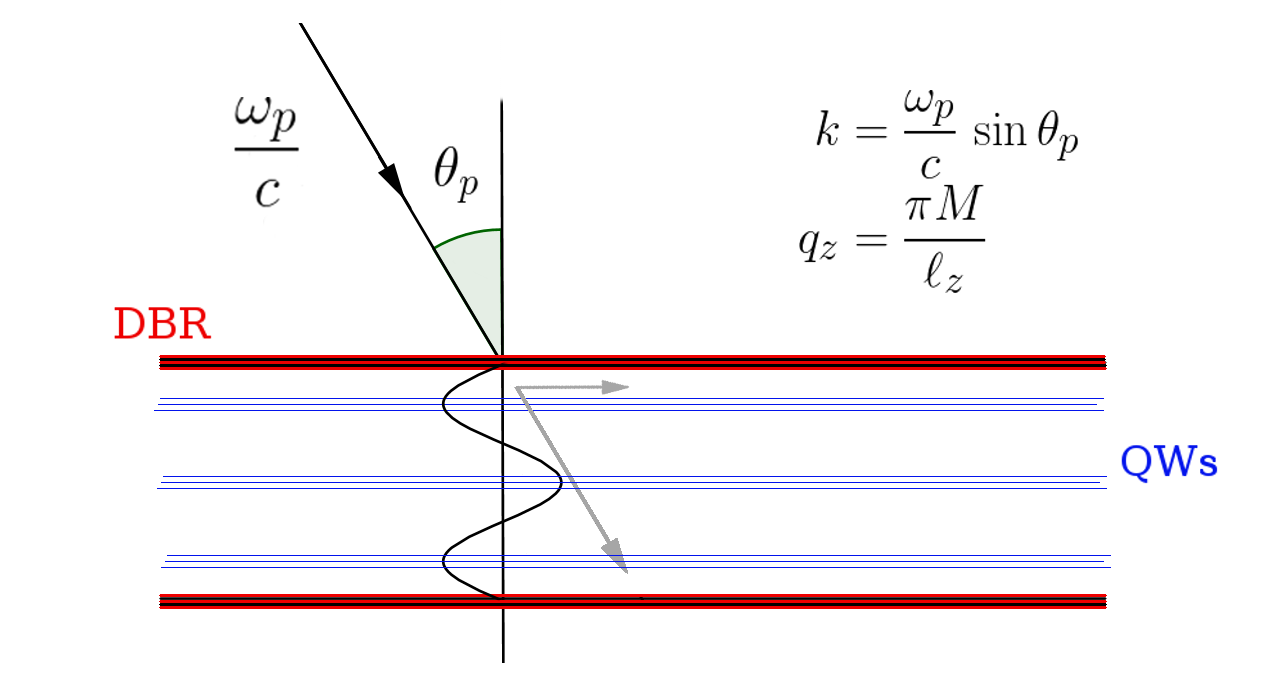
\includegraphics[height=.4\textheight]{pics/QW_field.png}}
    \end{figure}

    Massa del fotone dipendente dallo stato trasverso eccitato

    \begin{columns}
     \begin{column}{.5\textwidth}
      \begin{align*}
        \omega_C(k) &= \frac{c}{n_0}\sqrt{{q_z}^2 + k^2} \\
                &\simeq \omega_C^0 + \frac{\hbar k^2}{2m_C} &&
        \end{align*}
     \end{column}

     \begin{column}{.6\textwidth}
      \begin{figure}
       \fbox{
       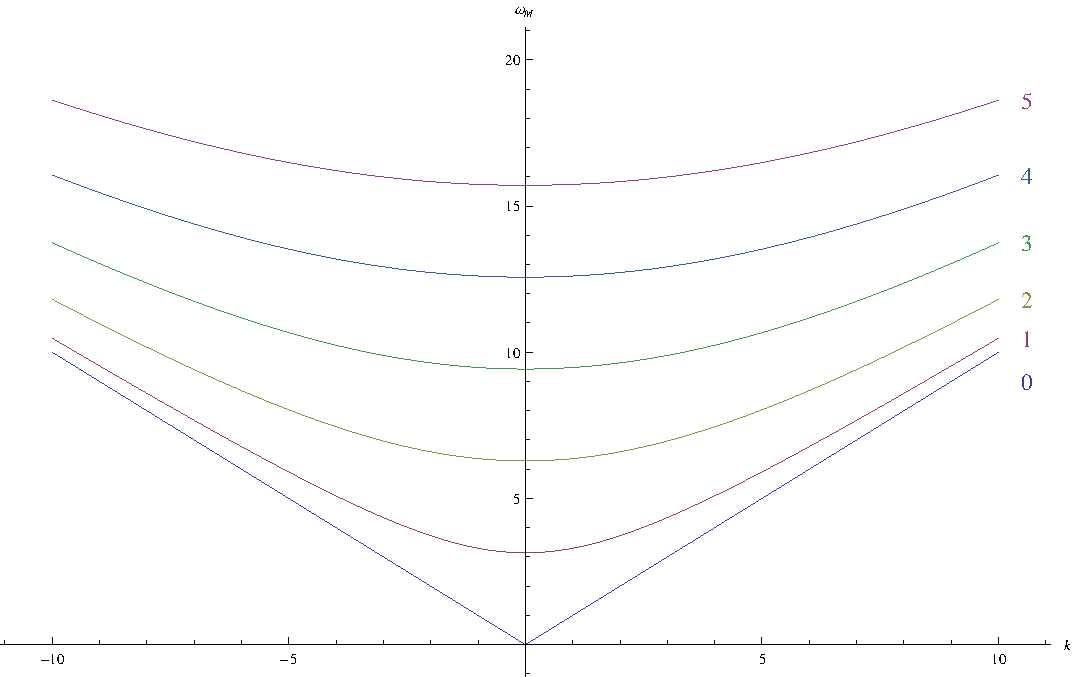
\includegraphics[width=.7\columnwidth]{pics/Photon_dispersion.pdf}}
      \end{figure}

     \end{column}


    \end{columns}


        
\end{frame}

 \begin{frame}{Quantum Wells}
 \alert{DA SISTEMARE}

 Buche/elettroni confinati lungo z \( \longrightarrow \) Eccitoni\\
 \vspace{10pt}
 Si comportano come bosoni\\
 Interagiscono con il campo laser nella cavità

 \begin{flalign*}
 \qquad &\omega_X(k) = \omega_X^0 + \frac{\hbar k^2}{2m_X} \\
  &V_{dip} \propto \vec d_X \cdot \vec E_{cav}
  &&
 \end{flalign*}
  \begin{figure}
  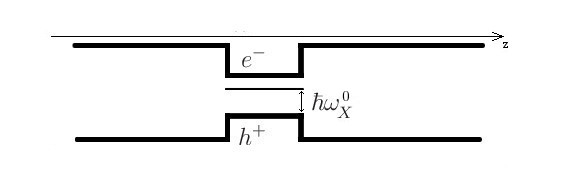
\includegraphics[width=\textwidth]{pics/QW.jpg}
 \end{figure}
   \end{frame}

 
\begin{frame}{Dinamica}


  Gradi di libertà sul piano $xy$
  \begin{itemize}
    \item { fotoni
   \begin{flalign*}
   \ham_{cav} = \intk \hbar \omega_C (k) \ \oa_C^\dagger \oa_C  &&
  \end{flalign*}
  }
      \item { eccitoni, con interaz. di dipolo (\(\Omega_r \ll \omega_C, \omega_X \))
 \begin{flalign*}
    \ham_{exc} = \intk \hbar \omega_X (k) \ \oa_X^\dagger \oa_X ~ + ~\hbar \Omega_R \left(\oa_C^\dagger \oa_X + \oa_X^\dagger \oa_C\right) &&
 \end{flalign*}
   }
  \end{itemize}
%     \onslide<\thebeamerpauses>{
%   \transdissolve<\thebeamerpauses>
 \begin{equation*}
  \boxed{
   \ham_{free} = \hbar \displaystyle \intk
      \begin{pmatrix} \oa_C^\dagger & \oa_X^\dagger \end{pmatrix}\,
      \begin{pmatrix} \omega_C & \Omega_R \\ \Omega_R & \omega_X \end{pmatrix}\,\begin{pmatrix}\oa_C \\ \oa_X \end{pmatrix}
      }
  \end{equation*}
%  }
\end{frame}

\begin{frame}{Polaritoni liberi}

\begin{equation*}
%\begin{align}
 \ham_{free} = \hbar \intk \omega_{LP} (k) \oa_{LP}^\dagger \oa_{LP} ~ + ~ \omega_{UP} (k) \oa_{UP}^\dagger \oa_{UP}
%\end{align}
\end{equation*}

\begin{minipage}{\textwidth}
\begin{columns}
\hskip.4cm
\footnotesize{
  \begin{column}{.45\textwidth}
   \begin{flalign*}
    \begin{cases}
        \oa_C = C\lp \ \oa\lp + C\up \ \oa\up \\
        \oa_X = X\lp \ \oa\lp + X\up \ \oa\up
     \end{cases}
     &&
   \end{flalign*}


   Coefficienti di Hopfield\\
   \( C_j (k) \approx X_j (k) \approx 1/2 \quad \text{@low }k\)

   \begin{equation*}
    \begin{align}
      &\displaystyle\omega_{ {\scriptstyle (UP,LP)} } (k) = \frac{\omega_C (k) + \omega_X (k)}{2} \\
                             &\pm \left[\Omega_R^2 + \left(\frac{\omega_C (k) - \omega_X (k)}{2}\right)^2\right]^{1/2}
    \end{align}
   \end{equation*}
   Dispersione
    \end{column}
  }
  \hfill
  \begin{column}{.55\textwidth}
   \begin{figure}[h]
    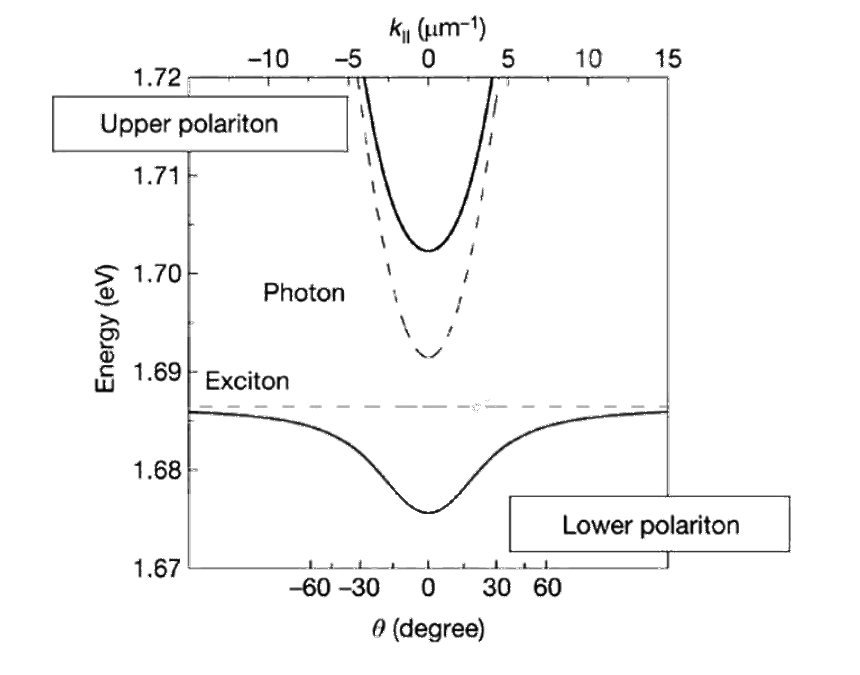
\includegraphics[scale=.2]{pics/polariton_dispersion.png}
   \end{figure}

  \end{column}
\end{columns}
\end{minipage}

\end{frame}



\subsection{Interazioni}

% You can reveal the parts of a slide one at a time
% with the \pause command:
\begin{frame}{Interazioni}
  %\transwipe[direction=270]
  Di carattere fotonico ed elettronico\\
  \footnotesize
  (le ultime sono dominanti)
  \normalsize
  \vskip.5cm
  \begin{itemize}
   \item {
   Nonlinearità ottiche
          \begin{flalign*}
           \chi^{(3)}{\vec E_{cav}}^4 \propto \chi^{(3)}(\oa_C^\dagger + \oa_C)^4 &&
          \end{flalign*}
   }
   \item{
   Scattering coulombiano tra eccitoni
            \begin{flalign*}
             \text{\large{$\tilde V$}} (k,k',q) \ \oa_X^\dagger (k+q) \oa_X^\dagger (k'-q) \oa_X (k') \oa_X (k) &&
            \end{flalign*}
   }
  \end{itemize}

  %\pause
        
\begin{columns}
 \begin{column}
  {.8\textwidth}
  \begin{equation*}
    \boxed{
      \ham_{int} = \intr \sum_{j=X,C} \frac{\hbar g_j}{2} \ \opsi_j^\dagger (r) \opsi_j^\dagger (r) \opsi_j (r) \opsi_j (r)
        }
   \end{equation*}
 \end{column}
  \begin{column}
  {.2\textwidth}
  \begin{itemize}
   \item $ka \ll 1$
   \item RWA
  \end{itemize}

 \end{column}


\end{columns}

\end{frame}

\subsection{Pumping \& losses}

\begin{frame}{Pompaggio laser}
  \begin{columns}
 \begin{column}
  {.45\textwidth}
    \begin{figure}[t]
    \flushleft
     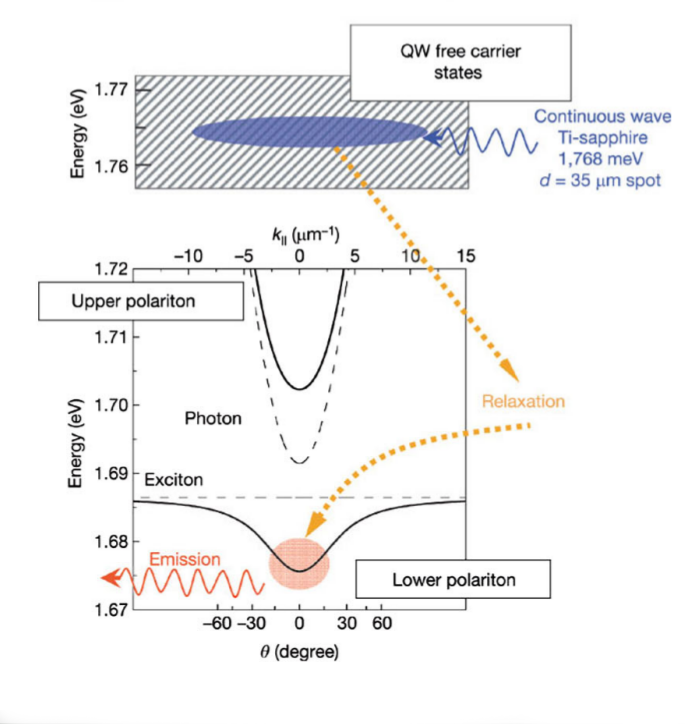
\includegraphics[scale=.18]{pics/incoherent.png}
    \end{figure}

 \end{column}
  \begin{column}
  {.55\textwidth}

     \textbf{Non coerente}\\
    % Alto detunig; Rilassamento; Altro...\\
     Fase del modo LP non fissata\\
    % Signal-idler condensate
     \vskip15pt
     \textbf{Coerente}\\
     Fase del condensato fissata dal laser\\
     si può includere nella dinamica
   \end{column}
\end{columns}

 \begin{equation*}
 \boxed{
    \begin{align*}
       \ham_{pump} &=\intr i\hbar \ \eta E_{inc} \ e^{ik_p r -i\omega_p t} \ \opsi_C^\dagger (r) +\hc \\
        &= \quad i\hbar \ \eta E_{inc} \ e^{-i\omega_p t} \ \oa_C^\dagger (k_p) +\hc
    \end{align*}
    }
 \end{equation*}
\end{frame}


\begin{frame}{Pompaggio laser}

\vspace{-.4cm}
{\footnotesize
\begin{columns}
\hskip10pt
\begin{column}{.4\textwidth}

Se l'ampiezza di interazione tra polaritoni è piccola rispetto allo splitting
%\( \big(|\omega_p - \omega\lp| \ll \omega\up - \omega\lp \big) \)
e il pump è accordato vicino al fondo della branca LP, la branca superiore è molto poco eccitata.\\
La trascuriamo, assieme a tutti i suoi termini nell'hamiltoniana:
\begin{flalign*}
  &
    \begin{cases}
        \opsi\up \approx 0 \\
        \opsi_C \approx C\lp \ \opsi\lp \\
        \opsi_X \approx X\lp \ \opsi\lp
     \end{cases}
  \\
  &\qquad\quad\Downarrow \\
  &\opsi\lp \approx C\lpsuper{*} \ \opsi_C + X\lpsuper{*} \ \opsi_X
   \end{flalign*}
   \end{column}
    \begin{column}{.6\textwidth}
      \begin{figure}
       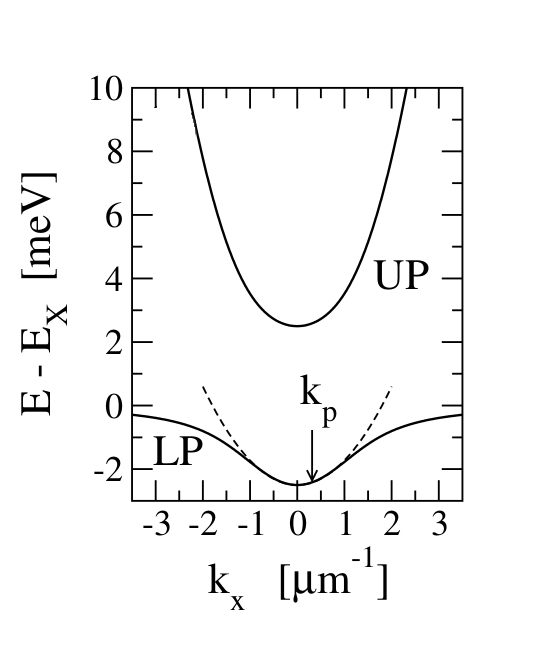
\includegraphics[scale=.25]{pics/LP_pump.png}
      \end{figure}
  \end{column}
 \end{columns}
}
\normalsize
\begin{align*}
  \ham = \ \hbar \intr & \opsi\lpsuper{\dagger} \ \big[ \omega\lp(-i\nabla) \big]\ \opsi\lp + \frac{g\lp}{2} \opsi\lpsuper{\dagger}  \opsi\lpsuper{\dagger}  \opsi\lp  \opsi\lp \\
        &+ \left( i F_p e^{ik_p r -i\omega_p t} \ \opsi\lpsuper{\dagger} + \hc \right)
\end{align*}

\end{frame}


\begin{frame}{Dissipazione}
Dovuta all'emissione attraverso gli specchi (trasmittività $\neq 0$)\\
smorzamento radiativo descritto con una master equation
%{\Large
\begin{equation*}
i\hbar \partial_t\ \rho = [H,\rho] + i\hbar \lind \rho
\end{equation*}
%}
con operatore di Lindblad 
\begin{flalign*}
\lind \rho = \intk \frac{\gamma_{{\scriptscriptstyle rad}}}{2} \left ( 2\oa_C\rho \oa_C^\dagger - \oa_C^\dagger \oa_C \rho - \rho \oa_C^\dagger \oa_C \right ) &&
\end{flalign*}
$\Rightarrow$ Ha l'effetto di inserire nell'equazione di Heisemberg per $\opsi_C$ un termine di smorzamento:
\[
 i \partial_t\, \opsi_C = \dots -i\frac{\gamma_{{\scriptscriptstyle rad}}}{2} \opsi_C
\]

% \begin{figure}
%        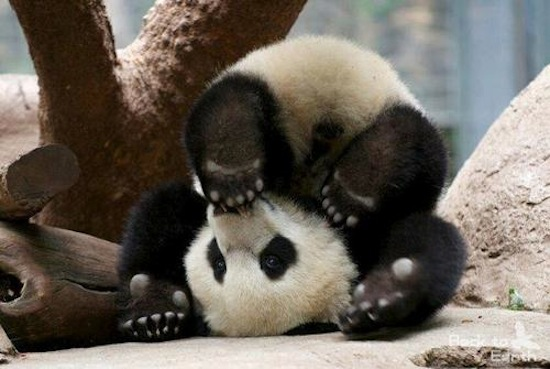
\includegraphics[scale=.3]{pics/Panda.jpg}
%        \caption{\footnotesize Qui ci rimetto il panda, che almeno lui mi fa compagnia}
%       \end{figure}

\end{frame}



\section{Teoria di campo medio}

\begin{frame}{Driven Dissipative GPE}
Mean Field: $\displaystyle \qquad\opsi\lp \longmapsto \left<\opsi\lp\right> \equiv \psi\lp$
% \[ i\hbar \partial_t \trcurl{\rho \opsi\lp} \approx i\hbar \partial_t \,\psi\lp
% \]

%{\centering
\vspace{5pt}{\footnotesize La sostituzione è esatta per i termini lineari, approssimata per l'interazione:}
\begin{equation*}
  \begin{cases}
             \left< \opsi^\dagger \opsi\, \opsi \right> \approx |\psi|^2 \psi \\
             \omega\lp (k) \approx {\omega\lp}^0 + \displaystyle\frac{\hbar k^2}{2m\lp} \\
           \end{cases}
\end{equation*}

            
% ddGPE
\ovalbox{
\begin{minipage}{\textwidth}
 \[
 i\partial_t \, \psi\lp = \left[ \omega\lp (-i\nabla) + g\lp |\psi\lp|^2 - i \frac{\gamma\lp}{2} \right]\, \psi\lp + i F_p e^{ik_pr - \omega_p t}
 \]
 \vskip0pt
\end{minipage}
}

\begin{flalign*}
 \begin{cases}
  m\lp = m_C/|C\lp|^2 \qquad &g\lp = |X\lp|^2 \,g_X + |C\lp|^2 \,g_C \\
  \gamma\lp = |C\lp|^2 \gamma_{{\scriptscriptstyle rad}} \qquad &F_p = C\lp\, \eta E_{inc}
 \end{cases}
 &&
\end{flalign*}

\end{frame}

\subsection{Stato stazionario}

\begin{frame}{Stato stazionario}
%\def\number{1}

\ifnum\number=1
{
\documentclass{article}
\usepackage[utf8]{inputenc}

\title{panda}
\author{Carmelo Mordini}
\date{May 2014}

\usepackage[utf8]{inputenc} % for writing other that basic characters
\usepackage[italian]{babel}
\usepackage{amsmath}
\usepackage{graphicx}
\usepackage{caption}
\usepackage{subcaption}

\begin{document}
}
\fi

\begin{figure}[!ht]
        \centering
        \subfloat[Panda]{
                
\includegraphics[trim=0.3cm 0cm 0cm 0cm, clip=true, 
                                width=.4\linewidth]
                                {files/pandabear/panda.jpg}
                       }
        \hfill
        \subfloat{
        \centering
        {\(\Rightarrow\)}
        }
        \hfill
        \subfloat[Polar bear]{
                \centering
                
\includegraphics[trim=0cm 0cm 0cm 0cm, clip=true, 
                                width=.4\linewidth]
                                {files/pandabear/polarbear.jpg}
                       }
        \caption[The panda-polar bear relationship ]
                {It is not widely known that the panda becomes a polar bear 
                when dressing up in the winter camouflage suite!}
        \label{fig: pentagram}
\end{figure}

\ifnum\number=1
{ \end{document}
}

Soluzione stazionaria: \( \psi\lpsuper{0}(r,t) = \psi\sts \ e^{ik_pr - i\omega_p t}  \leftarrow\) \alert{phase locking}

\[
 \left( \omega_p - \omega\lp (k_p) - g\lp |\psi\sts|^2 + i \frac{\gamma\lp}{2} \right)\, \psi\sts = i F_p
\]



\begin{figure}
 \end{figure}

La stabilità delle soluzioni si valuta linearizzando attorno alla soluzione $\psi\lpsuper{0}$, e dipende dall'intensità del laser di pump e dal detuning \(\Delta \omega_p = \omega_p - \omega\lp(k_p)\):
% \begin{figure}
% 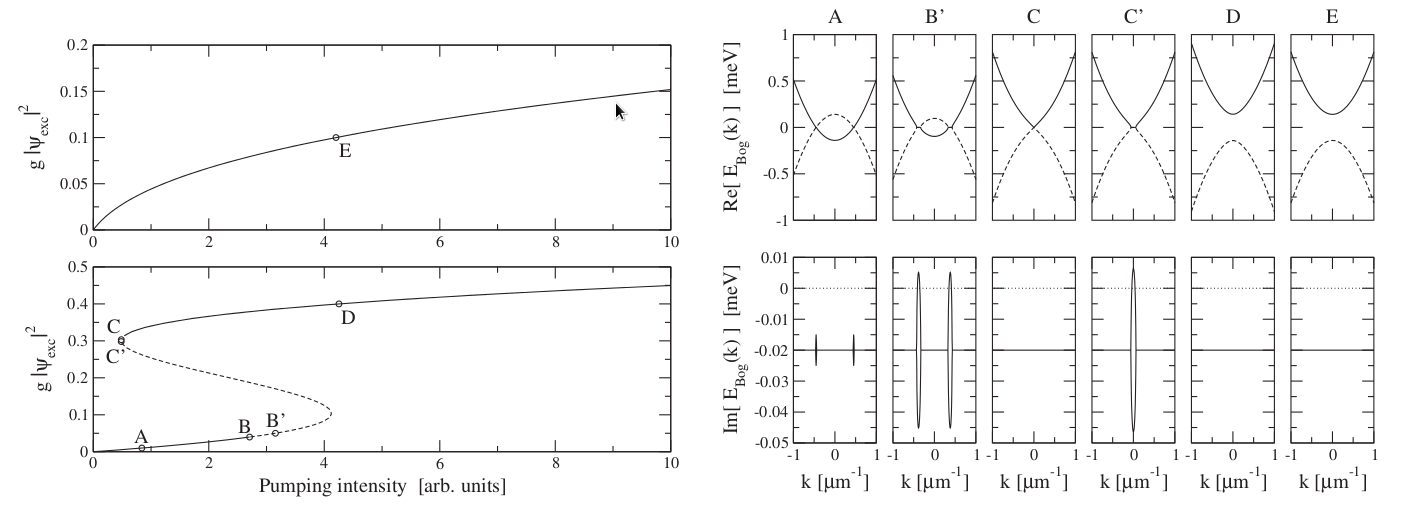
\includegraphics[width=\textwidth]{pics/Shapevspump-and-Spectra.png}
% \end{figure}
\begin{columns}[t]
 \begin{column}{.5\textwidth}
  \begin{figure}
   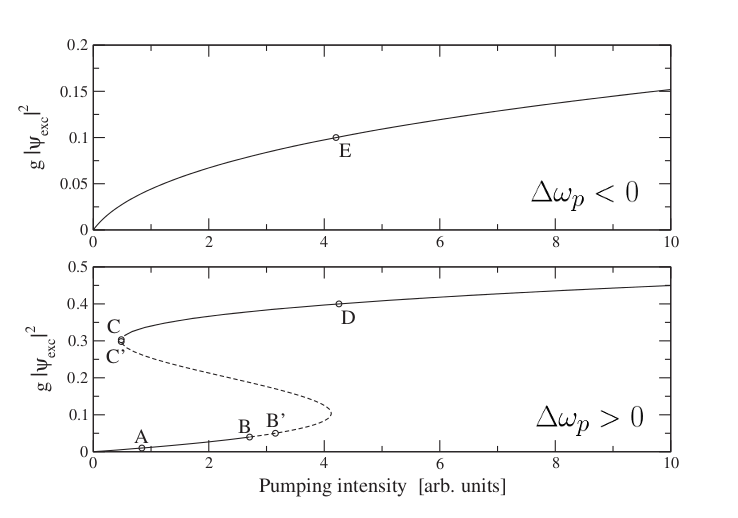
\includegraphics[width=\columnwidth]{pics/Shapevspump.png}
   %\smallcaption{\(\Delta\omega_p <0\) (top) vs \(\Delta\omega_p >0\) (bottom)}
  \end{figure}

 \end{column}

 \begin{column}{.5\textwidth}
  \begin{figure}
   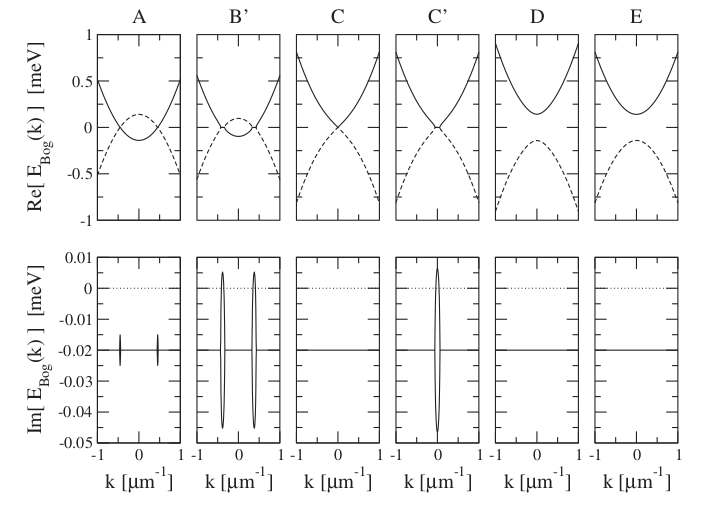
\includegraphics[width=\columnwidth]{pics/Spectra.png}
  % \smallcaption{Spettro di Bogoliubov nei due casi}
  \end{figure}
 \end{column}

\end{columns}


\end{frame}

\subsection{Spettro delle eccitazioni}

\begin{frame}{Spettro delle eccitazioni}
Soluzione stazionaria: \( \psi\lp(r,t) = \left(\psi\sts + \delta\psi (r,t) \right)e^{ik_pr - i\omega_p t} \)\\
Al I ordine in \(\delta\psi\), lo spettro delle eccitazioni (modi di Bogoliubov) si ricava con un procedimento analogo al caso di un gas di bosoni all'equilibrio
{\footnotesize
\begin{flalign*}
 \bvec{\delta \psi} = {\big( \delta\psi \; , \; {\delta\psi}^* \big)}^T \\
 \\
 i \partial_t\, \bvec{\delta\psi} = \mathcal{L}\bog \cdot \bvec{\delta\psi}
 \end{flalign*}


}
% {\footnotesize
% \[
%  \begin{pmatrix}
%   \omega\lp (k) + 2 g\lp |\psi\sts|^2 -i\frac{\gamma\lp (k)}{2}       &\hspace{-1cm}  g\lp{\psi\sts}^2 \\
%   \\
%   \\ \hspace{-1.8cm}- g\lp{{\psi\sts}^*}^2    & \hspace{-1.8cm}       2\omega_p -\left(\omega\lp (2k_p-k) + 2g\lp|\psi\sts|^2\right) -i\frac{\gamma\lp (2k_p-k)}{2}
%  \end{pmatrix}
% \]
% }

\[
 \omega\bogsuper{\pm} = \omega_p + \delta k \cdot v_p -i\frac{\gamma\lp}{2} \pm \sqrt{\left(2 g\lp |\psi\sts|^2 + \eta_{\delta k} - \Delta_p\right)\left(\eta_{\delta k} - \Delta_p\right)}
\]
{\footnotesize
dove i parametri di controllo entrano in
\begin{flalign*}
 \begin{cases}
    \delta k = k-k_p \qquad \eta_{\delta k}= \frac{\hbar {\delta k}^2}{2 m\lp} \\
    \Delta_p = \omega_p - \omega\lp(k_p) - g\lp |\psi\sts|^2
 \end{cases}
 &&
\end{flalign*}
}

 \end{frame}


\section{Superfluidità}

\subsection{Resonant Raileigh Scattering}

\begin{frame}{Perturbazione}
 \end{frame}

\subsection{Criterio di Landau}
\subsection{Verifica sperimentale}

\begin{frame}{Video}
\movie[borderwidth=.6pt,
      height=.5\textheight,
      width=.5\textwidth,
      ]%externalviewer]
      {}{movies/cherexp.mp4}
      \\
Hello
% \begin{figure}
%  \includemedia[
% activate=pageopen,
% deactivate=pageclose,
% width=200pt, height=150pt,
% addresource=weyllaw.mp4,
% flashvars={
% src=weyllaw.mp4
% &loop=false
% &autoPlay=true
% }
% ]{movies/cherexp.mp4}
% \end{figure}


\end{frame}



% Placing a * after \section means it will not show in the
% outline or table of contents.


\section*{Summary}

\begin{frame}{Summary}
  Ciao
\end{frame}



% All of the following is optional and typically not needed.
\appendix
\section<presentation>*{\appendixname}
\subsection<presentation>*{For Further Reading}

\begin{frame}[allowframebreaks]
  \frametitle<presentation>{For Further Reading}

  \begin{thebibliography}{10}

  \beamertemplatebookbibitems
  % Start with overview books.

  \bibitem{Author1990}
    A.~Author.
    \newblock {\em Handbook of Everything}.
    \newblock Some Press, 1990.


  \beamertemplatearticlebibitems
  % Followed by interesting articles. Keep the list short.

  \bibitem{Someone2000}
    S.~Someone.
    \newblock On this and that.
    \newblock {\em Journal of This and That}, 2(1):50--100,
    2000.
  \end{thebibliography}
\end{frame}

\end{document}
